\documentclass[a4paper,10pt,fleqn]{article}

\usepackage{a4wide,amsmath,amsthm,amssymb,bbm,fancyhdr}
\usepackage{ifthen,color,enumerate,comment,dsfont,pdfsync,framed,todonotes,enumitem}
\newboolean{corrige}
\setboolean{corrige}{true}

\newcommand{\titre}[1]{\textbf{\textsc{#1}}}

\RequirePackage[T1]{fontenc}

\usepackage[latin1]{inputenc}
\usepackage{graphicx}
\usepackage{dsfont}
\newcommand{\thisyear}{}
\usepackage{enumitem}
\newcommand{\eqsp}{\,}
\newcommand{\R}{\ensuremath{\mathbb{R}}}
\newcommand{\calF}{\mathcal{F}}
\newcommand{\N}{\mathbb{N}}
\newcommand{\rset}{\ensuremath{\mathbb{R}}}
\renewcommand{\P}{\ensuremath{\operatorname{P}}}
\newcommand{\bP}{\mathbb{P}}
\newcommand{\E}{\ensuremath{\mathbb{E}}}
\newcommand{\rme}{\ensuremath{\mathrm{e}}}
\newcommand{\calH}{\ensuremath{\mathcal{H}}}
\newcommand{\xset}{\ensuremath{\mathsf{X}}}
\newcommand{\V}{\ensuremath{\mathbb{V}}}
\newcommand{\Sb}{\ensuremath{\mathbb{S}}}
\newcommand{\gaus}{\ensuremath{\mathcal{N}}}
\newcommand{\HH}{\ensuremath{\mathcal{H}}}
\newcommand{\F}{\ensuremath{\mathcal{F}}}
\newcommand{\W}{\ensuremath{\mathcal{W}}}
\newcommand{\X}{\ensuremath{\mathcal{X}}}
\newcommand{\1}{\ensuremath{\mathbbm{1}}}
\newcommand{\dlim}{\ensuremath{\stackrel{\mathcal{L}}{\longrightarrow}}}
\newcommand{\plim}{\ensuremath{\stackrel{\mathrm{P}}{\longrightarrow}}}
\newcommand{\PP}{\ensuremath{\mathbb{P}}}
\newcommand{\p}{\ensuremath{\mathbb{P}}}
\newcommand{\eps}{\varepsilon}
\newcommand{\bE}{\mathbb{E}}
\newcommand{\pa}[1]{\left(#1\right)}
\newcommand{\hatk}{\widehat K}
\newcommand{\f}{\varphi}
\newcommand{\Id}{\textsf{Id}}
\newcommand{\bfU}{\mathbf{U}}
\newcommand{\bfX}{\mathbf{X}}
\newcommand{\bfs}{\mathbf{\Sigma}}
\newcommand{\bfA}{\mathbf{A}}
\newcommand{\bfV}{\mathbf{V}}
\newcommand{\bfB}{\mathbf{B}}
\newcommand{\bfI}{\mathbf{I}}
\newcommand{\bfD}{\mathbf{D}}
\newcommand{\bfK}{\mathbf{K}}
\newcommand{\argmin}{\mathop{\textrm{argmin}}}
\newcommand{\argmax}{\mathop{\textrm{argmax}}}
\newcommand{\crit}{\mathop{\textrm{crit}}}
\newcommand{\C}{\mathcal{C}}
\newcommand{\pc}{\pi_{\mathcal{C}}}


% Style
%\pagestyle{fancyplain}
\renewcommand{\sectionmark}[1]{\markright{#1}}
\renewcommand{\subsectionmark}[1]{}
%\lhead[\fancyplain{}{\thepage}]{\fancyplain{}{\footnotesize {\sf
%MAT4506 Introduction to Machine Learning  %/ \rightmark
%}}}
%\rhead[\fancyplain{}{\footnotesize {\sf MAT4506 Introduction to machine learning, \thisyear %/ \rightmark
%}}]{\fancyplain{}{\thepage}}


\newtheorem{theorem}{Theorem}

%% Titre
%\title{{\bf Machine learning}}
%\author{{\em Logistic regression}}
%\date{}


\begin{document}

\noindent Machine learning \hfill ISUP - Sorbonne Universit\'e \\
 2022-2023

\noindent\hrulefill

\begin{center}
\textsc{Logistic regression}
\end{center}
\hrulefill

\medskip



\section{Warm-up}
The \emph{logistic model} assumes that the random variables  $(X,Y)\in \rset^d\times\{0,1\}$ are such that
$$
\bP(Y=1|X)={\exp\left(\langle \beta^*,X\rangle\right)\over 1+\exp\left(\langle \beta^*,X\rangle\right)}\eqsp,
$$
with $\beta^*\in\mathbb{R}^d$. In this case,  $\bP(Y=1|X)>1/2$ if and only if $\langle \beta^*,X\rangle>0$, so
the frontier between $\left\{x\eqsp;\eqsp h_{*}(x)=1\right\}$ and $\left\{x\eqsp ;\eqsp h_{*}(x)=0\right\}$ is an hyperplane, with orthogonal
direction $\beta^*$. 
\begin{enumerate}

	\item In this question only,  $\beta^* = (\beta_0,\beta_1)\in \rset^2$ and $X_i = (1,x_i)$ for all $1\leqslant i \leqslant n$.

\begin{enumerate}
\item Provide the value $x_*$ of $x_i$ such that $\mathbb{P}(Y_i=1 | X_i) = 1/2$. The logistic Bayes classifier is therefore defined by $h_*(X_i) = 1$ if and only if $x_i>x_*$. 
\item Another classifier could be defined by choosing a threshold $\tilde p\in(0,1)$ and defining $\tilde h(X_i) = 1$ if and only if $\mathbb{P}(Y_i=1 | X_i) > \tilde p$.  Provide $\tilde x$ such that $\tilde h(X_i) = 1$ if and only if $x_i>\tilde x$. Explain a practical interest to choose $\tilde p < 1/2$.
\end{enumerate}
	\item The usual logistic regression classifier is defined by $h_n:x\mapsto 1$ is $x^\top\hat\beta_n >0$ and $0$ otherwise, where $\hat \beta_n$ is an estimator of $\beta$. Therefore $h_n(X) =1$ if and only if $\mathbb{P}(Y=1|X)>1/2$. Other classifiers can be defined by setting $h_n(X) =1$ if and only if $\mathbb{P}(Y=1|X)>p_*$ for a chosen $p_*\in(0,1)$. Two classifiers were built with $p_* = 0.5$ and $p_* = 0.2$, associate each classifier with its point on  ROC curve displayed above.

\begin{figure}[h!]
\label{fig:roc}
\centering
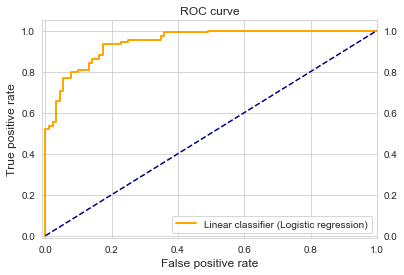
\includegraphics[scale = .45]{roc.png}
\end{figure}
	
\end{enumerate}

\section{Softmax regression}
Assume that the observation $Y$ takes values in $\{1,\ldots,M\}$ and that $X\in\mathbb{R}^d$. The negative loglikelihood to be minimized to estimate the parameters of the model is given by:
$$
\theta \mapsto \ell^{\mathrm{multi}}_n(\theta)= -\frac{1}{n} \sum_{i=1}^n\sum_{k=1}^{M} \1_{Y_i=k}\log \mathbb{P}_{\theta}(Y_i = k | X_i)\,,
$$
where $\{(X_i,Y_i)\}_{1\leqslant i\leqslant n}$ are i.i.d. observations with the same law as $(X,Y)$. 

\begin{enumerate}
\item Explain the construction of $\mathbb{P}_{\theta}(Y_i = k | X_i)$, $1\leqslant i\leqslant n$ for a softmax regression model with parameters $\omega_m\in\mathbb{R}^d$ for $1\leqslant m  \leqslant M$.
\item In the setting  of the softmax regression function, compute $\theta \mapsto \nabla_\theta \ell^{\mathrm{multi}}_n(\theta)$.
\end{enumerate}


\section{Maximum likelihood estimation}
The unknown parameter $\beta^*$ may be estimated  by maximizing the conditional likelihood of $Y$ given $X$
$$
\widehat \beta_n\in\mathrm{argmax}_{\beta\in\mathbb{R}^{d}}
\prod_{i=1}^n \left[ \left( \frac{\exp\left(\langle
	\beta,x_{i}\rangle\right)}{1+\exp\left(\langle
	\beta,x_{i}\rangle\right)}\right)^{Y_{i}}
\left(\frac{1}{1+\exp\left(\langle
	\beta,x_{i}\rangle\right)}\right)^{1- Y_{i}} \right] ,
$$
to define the empirical classifier
$$
\widehat h_{n}: x \mapsto \1_{\langle \widehat\beta_n,x\rangle>0}\eqsp.
$$
In the following, $\{(x_i,Y_i)\}_{1\leqslant i\leqslant n}$ are assumed to be i.i.d. with the same distribution as $(X,Y)$.
\begin{enumerate}
\item Compute the gradient and the Hessian $H_{n}$ of
$$
\ell_{n}:\beta \mapsto -\sum_{i=1}^n\left[Y_{i}\langle x_{i},\beta\rangle-\log(1+\exp(\langle x_{i},\beta\rangle))\right]\eqsp.
$$
What can be said about the function $\ell_{n}$ when for all $\beta\in\rset^d$, $H_{n}(\beta)$ is nonsingular? This assumption is supposed to hold in the following questions.
\item Prove that there exists $\widetilde \beta_n\in\rset^d$ such that $\|\widetilde \beta_n-\beta^*\|\leq \|\widehat \beta_n-\beta^*\|$ and
$$
\widehat \beta_n-\beta^*=-H_{n}(\widetilde \beta_n)^{-1}\nabla \ell_{n}(\beta^*)\eqsp.
$$
\end{enumerate}
In the following it is assumed that the $(x_{i})_{1\leqslant i\leqslant n}$ are uniformly bounded, $\widehat \beta_n\to \beta^*$ a.s. and that there exists a continuous and nonsingular function $H$ such that $n^{-1}H_{n}(\beta)$ converges to $H(\beta)$, uniformly in a ball around $\beta^*$.
\begin{enumerate}  \setcounter{enumi}{2}
\item Define for all $1\leqslant i \leqslant n$, $p_{i}(\beta)=e^{\langle x_{i},\beta\rangle}/ \left(1+e^{\langle x_{i},\beta\rangle}\right)$. Check that
\begin{align*}
\bE \left[e^{-n^{-1/2}\langle t,\nabla\ell_{n}(\beta^*)\rangle}\right]& =\prod_{i=1}^n \left({1-p_{i}(\beta^*)+p_{i}(\beta^*)e^{\langle t,x_{i}\rangle/\sqrt{n}}}\right) e^{-p_{i}(\beta^*)\langle t,x_{i}\rangle/\sqrt{n}}\eqsp, \\
&=\exp\left(\frac{1}{2}t^T\left(n^{-1}H_{n}(\beta^*)\right)t+O(n^{-1/2})\right)\eqsp.
\end{align*}
\item What is the asymptotic distribution of $-n^{-1/2}\nabla\ell_{n}(\beta^*)$ and of $\sqrt{n}(\widehat \beta_n-\beta^*)$?
\item For all $1\leqslant j \leqslant d$ and all $\alpha\in(0,1)$, propose a confidence interval $\mathcal{I}_{n,\alpha}$ such that $\beta^*_{j}\in \mathcal{I}_{n,\alpha}$ with asymptotic probability $1-\alpha$.
\end{enumerate}


\end{document} 